% !TEX program = xelatex
\documentclass[11pt,a4paper]{article}
\usepackage{fontspec}
\setmainfont{TeX Gyre Termes}
\usepackage[a4paper,margin=23mm,headheight=16pt]{geometry}
\usepackage{amsmath,amssymb,booktabs,graphicx,xcolor,fancyhdr,lastpage,hyperref,enumitem,caption}
\definecolor{CoursePurple}{HTML}{5C2267}
\hypersetup{colorlinks=true,linkcolor=CoursePurple,urlcolor=CoursePurple,pdftitle={DDA5001 Homework 3}}
\pagestyle{fancy}\fancyhf{}
\fancyhead[L]{\small DDA5001 Machine Learning}\fancyhead[R]{\small Homework 3}
\fancyfoot[R]{\small\thepage/\pageref*{LastPage}}
\setlength{\parindent}{0pt}\setlength{\parskip}{5pt}\setlength{\emergencystretch}{3em}
\captionsetup{font=small,labelfont=bf,skip=4pt}
\graphicspath{{images/}}
\newcommand{\R}{\mathbb R}
\begin{document}
\begin{center}{\Large\bfseries\color{CoursePurple}DDA5001 Homework 3}\\[4pt]
The Chinese University of Hong Kong, Shenzhen
\end{center}
\noindent\rule{\linewidth}{0.8pt}
\section*{Problem 1(a): Regularization and five-fold validation}
For a fit on $m$ observations, let $X\in\R^{m\times9}$ have columns $1,x,\ldots,x^8$. The objective, including a penalty on the intercept, is
\[
J_\lambda(\theta)=\frac1m\|X\theta-y\|_2^2+\lambda\|\theta\|_2^2.
\]
Differentiating and setting the gradient to zero gives
\[
\nabla J_\lambda=\frac2mX^\top(X\theta-y)+2\lambda\theta=0,
\qquad (X^\top X+m\lambda I_9)\widehat\theta_\lambda=X^\top y.
\]
Thus
\[
\boxed{\widehat\theta_\lambda=(X^\top X+m\lambda I_9)^{-1}X^\top y.}
\]
For any nonzero $v$, $v^\top(X^\top X+m\lambda I)v=\|Xv\|^2+m\lambda\|v\|^2>0$ when $\lambda>0$. The solution is unique. The code evaluates this equation with \texttt{np.linalg.solve}, without explicitly forming an inverse; $m=10$ for the final fit.

The original CSV row IDs define validation folds
\[
V_1=\{6,0\},\ V_2=\{3,9\},\ V_3=\{2,1\},\
V_4=\{4,8\},\ V_5=\{5,7\}.
\]
For each of the 16 prescribed candidates, the supplied fitting routine trains on the eight remaining rows. The completed scoring function computes
\[
E_f(\lambda)=\frac12\sum_{i\in V_f}
  \bigl(f_{\widehat\theta_{\lambda,-f}}(x_i)-y_i\bigr)^2,\qquad
\mathrm{CV}(\lambda)=\frac15\sum_{f=1}^5 E_f(\lambda).
\]
Rows are never sorted or renumbered. Taking the first minimum over ascending candidates implements the exact-tie rule. The selected value is
\[
\boxed{\lambda^\star=0.01,\qquad \mathrm{CV}(\lambda^\star)=0.04826737.}
\]
\begin{center}
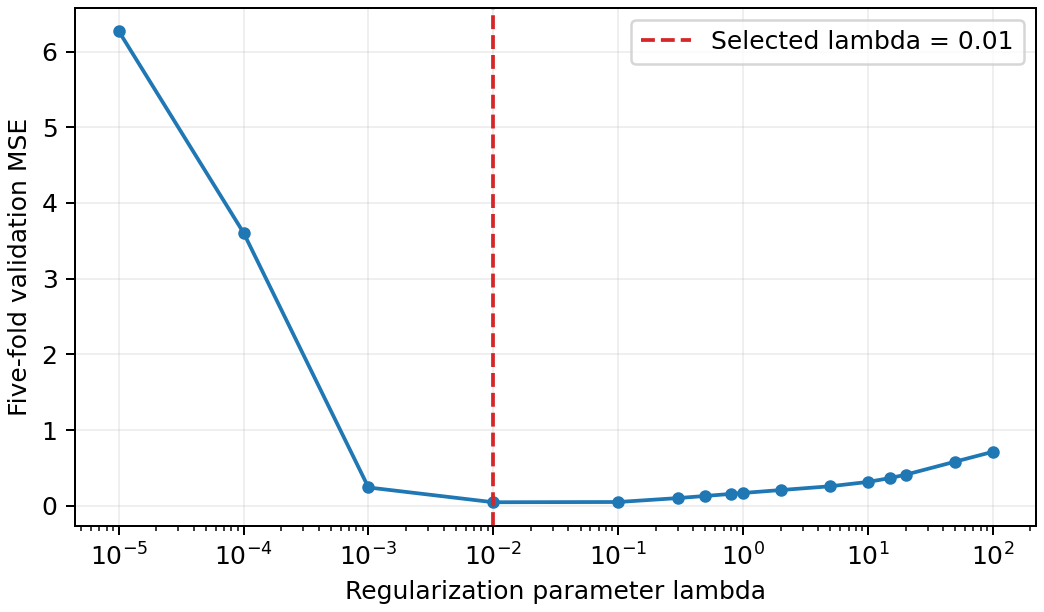
\includegraphics[width=.80\linewidth]{p1-validation.png}
\captionof{figure}{Five-fold mean validation MSE, with a logarithmic $\lambda$ axis.}
\end{center}

\clearpage
\section*{Problem 1(b): Refit and final evaluation}
After selecting $\lambda^\star$ using only training-set folds, the regularized model is refitted on all ten training rows. The baseline uses the supplied unregularized least-squares solver. Both models are then evaluated on the ten independent test observations.
\begin{center}
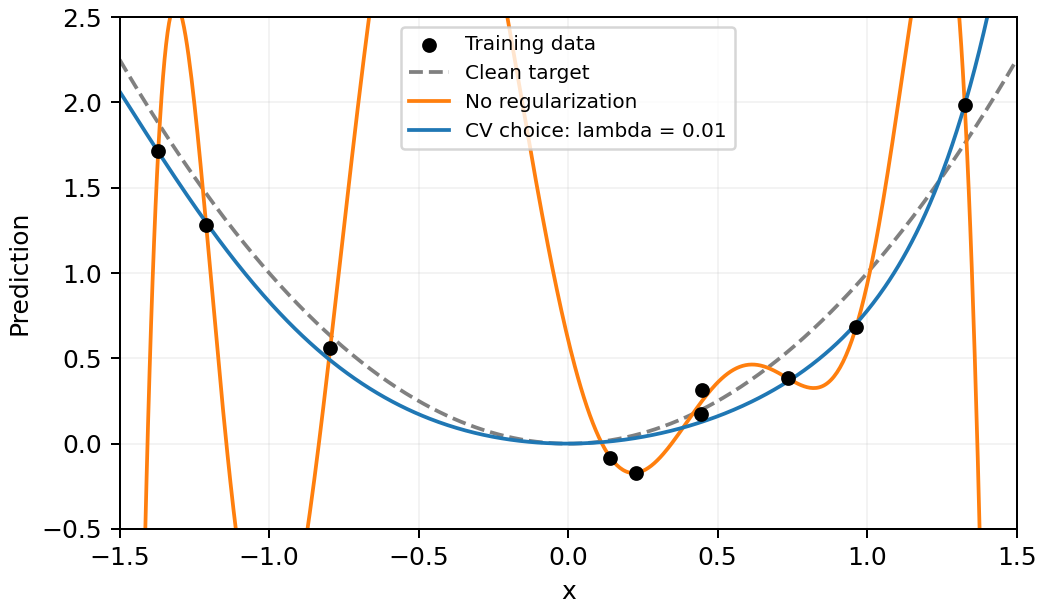
\includegraphics[width=.98\linewidth]{p1-fits.png}
\captionof{figure}{Degree-8 fits, the original training points and the clean target $x^2$. The prescribed display limits are $x\in[-1.5,1.5]$, $y\in[-0.5,2.5]$; parts of the unregularized curve extend beyond this window.}
\end{center}
\begin{center}
\begin{tabular}{lrr}
\toprule
Fit & Training MSE & Test MSE\\
\midrule
Unregularized ($\lambda=0$) & 0.00090436 & 2.08003393\\
Validation-selected ($\lambda=0.01$) & 0.00933397 & 0.04021308\\
\bottomrule
\end{tabular}
\end{center}
The unregularized fit closely matches the noisy training observations but oscillates strongly between them, whereas regularization increases training MSE and substantially reduces test MSE in this run. The selected curve follows the clean quadratic trend more closely, illustrating a useful reduction in overfitting rather than a guarantee that every regularizer improves prediction. Validation chooses $\lambda$ without using test outcomes, so the test set remains a separate final assessment instead of becoming another tuning set.

\textbf{Implementation and checks.} Only \texttt{fit\_ridge\_final} and \texttt{score\_and\_select\_cv} in \texttt{p1/p1.py} were completed. A small analytic check with $X=I_2$, $y=(2,4)^\top$ and $\lambda=0.5$ returns $(1,2)^\top$, checking the factor $m$ and the penalty on every coordinate. A synthetic exact tie selects the smaller candidate. These checks supplement, rather than replace, the supplied-data experiment.

\textbf{Data and outputs.} The two CSVs are unchanged from the teacher package. Running \texttt{p1.py} produces the complete candidate-by-fold table in \texttt{cross\_validation.csv}, a \texttt{summary.json} with coefficients and errors, and the figures shown here. These numerical files are generated outputs; none of the reported errors uses the clean curve in place of the noisy observed targets.

\clearpage
\section*{Problem 2(a): Centered PCA and eigenfaces}
The 400 original $112\times92$ faces are ordered by subject $1,\ldots,40$, then image $1,\ldots,10$. The supplied loader divides pixels by 255; the completed matrix constructor flattens each image in row-major order without further normalization:
\[
X=[x_1,\ldots,x_{400}]\in\R^{10304\times400},\quad
\mu=\frac1{400}X\mathbf1,\quad X_c=X-\mu\mathbf1^\top.
\]
The code uses the thin SVD
\[
X_c=U\Sigma V^\top,\qquad U\in\R^{10304\times400},
\]
with singular values in descending order. The first $k$ columns of $U$ form an orthonormal basis $A_k$ minimizing the rank-$k$ reconstruction error. No $10304\times10304$ covariance matrix is formed.
\begin{center}
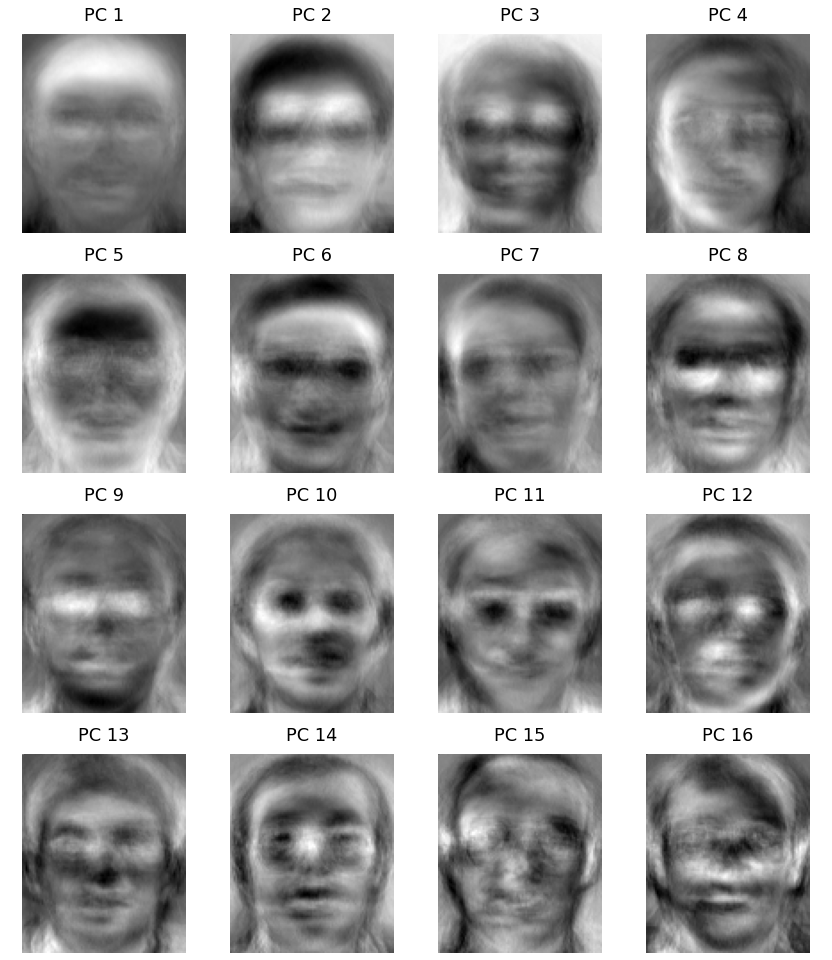
\includegraphics[height=16.4cm]{p2-eigenfaces.png}
\captionof{figure}{First 16 eigenfaces in descending singular-value order, read left to right and top to bottom. Display signs follow the supplied convention; reversing a basis vector's sign does not change its subspace or reconstruction.}
\end{center}

\clearpage
\section*{Problem 2(b): Coordinates and reconstruction}
For each $k$, the completed function returns
\[
\Theta_k=A_k^\top(X-\mu\mathbf1^\top)\in\R^{k\times400},\qquad
\widehat X_k=\mu\mathbf1^\top+A_k\Theta_k.
\]
\begin{center}
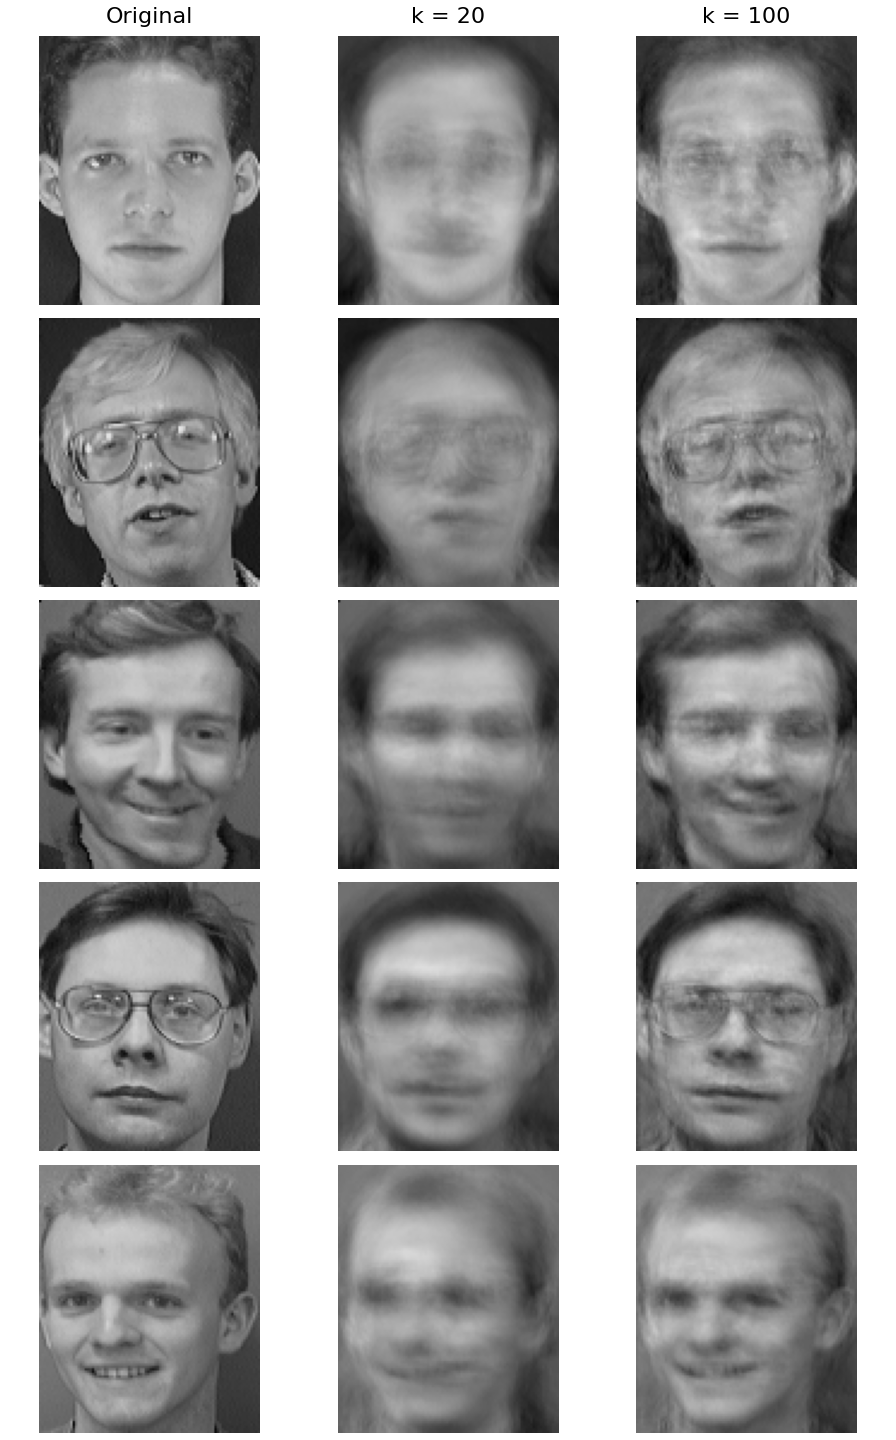
\includegraphics[height=16.0cm]{p2-reconstruction.png}
\captionof{figure}{Image 1 of subjects 1--5, in row order (columns $0,10,20,30,40$ of $X$). Each row shows the original, $k=20$ reconstruction and $k=100$ reconstruction.}
\end{center}
\begin{center}
\begin{tabular}{cr}
\toprule
Components $k$ & Whole-dataset MSE $\|\widehat X_k-X\|_F^2/(10304\cdot400)$\\
\midrule
20 & 0.00734732\\
100 & 0.00271577\\
\bottomrule
\end{tabular}
\end{center}
Increasing $k$ from 20 to 100 preserves more detail around the eyes, hair and glasses and lowers the measured reconstruction error. The nested PCA subspaces retain more variation, but require five times as many coordinates per face. MSE is computed on all pixels of all 400 unclipped reconstructions; only the displayed images are clipped to $[0,1]$.

\clearpage
\section*{Problem 3(a): Prediction before running}
The following prediction was recorded in the AI-assisted workflow before model checks or training. Two affine layers without an activation collapse to
\[
W_2(W_1x+b_1)+b_2=(W_2W_1)x+(W_2b_1+b_2).
\]
Therefore B remains affine in $x$. Its effective matrix has rank at most 64, but every $10\times784$ matrix has rank at most 10; width 64 is sufficient to represent every matrix available to A. More explicitly, choose the first ten rows of $W_1$ to be any desired $W$, set its other rows to zero, and take $W_2=[I_{10}\ 0]$, $b_1=0$, $b_2=b$.

A and B consequently have the same input-to-logit function class, although their parameterization and optimization trajectories may differ. ReLU allows C to use different affine pieces for different activation patterns, adding nonlinear representational capacity that may help with digits. Comparing B and C keeps width, depth, biases and parameter counts fixed, isolating the architectural addition of ReLU under the prescribed training protocol; no exact accuracy or universal ranking was predicted.

\section*{Problem 3(b): Model construction}
The only changes to \texttt{p3/p3.py} are the three model constructors:
\begin{center}
\small
\begin{tabular}{clrr}
\toprule
Model & Layers, in forward order & Output & Parameters\\
\midrule
A & Linear$(784,10)$ & 10 logits & 7,850\\
B & Linear$(784,64)$; Linear$(64,10)$ & 10 logits & 50,890\\
C & Linear$(784,64)$; ReLU; Linear$(64,10)$ & 10 logits & 50,890\\
\bottomrule
\end{tabular}
\end{center}
Every linear layer includes a bias. An input batch is $N\times784$; B/C produce an intermediate $N\times64$ tensor, then $N\times10$ logits. C applies $\max(z,0)$ elementwise only after the first affine layer. There is no output ReLU or Softmax: the supplied cross-entropy function consumes raw scores. The counts are $784\cdot10+10$ for A and $(784\cdot64+64)+(64\cdot10+10)$ for B/C; ReLU has no trainable parameters.

\textbf{Checks.} The supplied \texttt{--check-models} command returned finite outputs of shape $(2,10)$ with the counts above. Additional automated checks inspected the actual layer types and biases and confirmed that B agrees with its collapsed affine formula in float64 at tolerance $10^{-12}$.

\textbf{Fixed experiment.} The supplied split has 6,000 training, 2,000 validation and 2,000 test images, class-balanced with seed 666. The unchanged framework trains for 30 epochs using minibatches of 128, SGD with momentum 0.9, learning rate 0.1, no weight decay, and training seed 666. It uses one CPU thread and deterministic PyTorch algorithms. Epoch 0 is an untrained plotted baseline; eligible checkpoints are epochs 1--30. The checkpoint and model choice use validation cross-entropy only, before test evaluation.

\clearpage
\section*{Problem 3(c): Results and interpretation}
\begin{center}
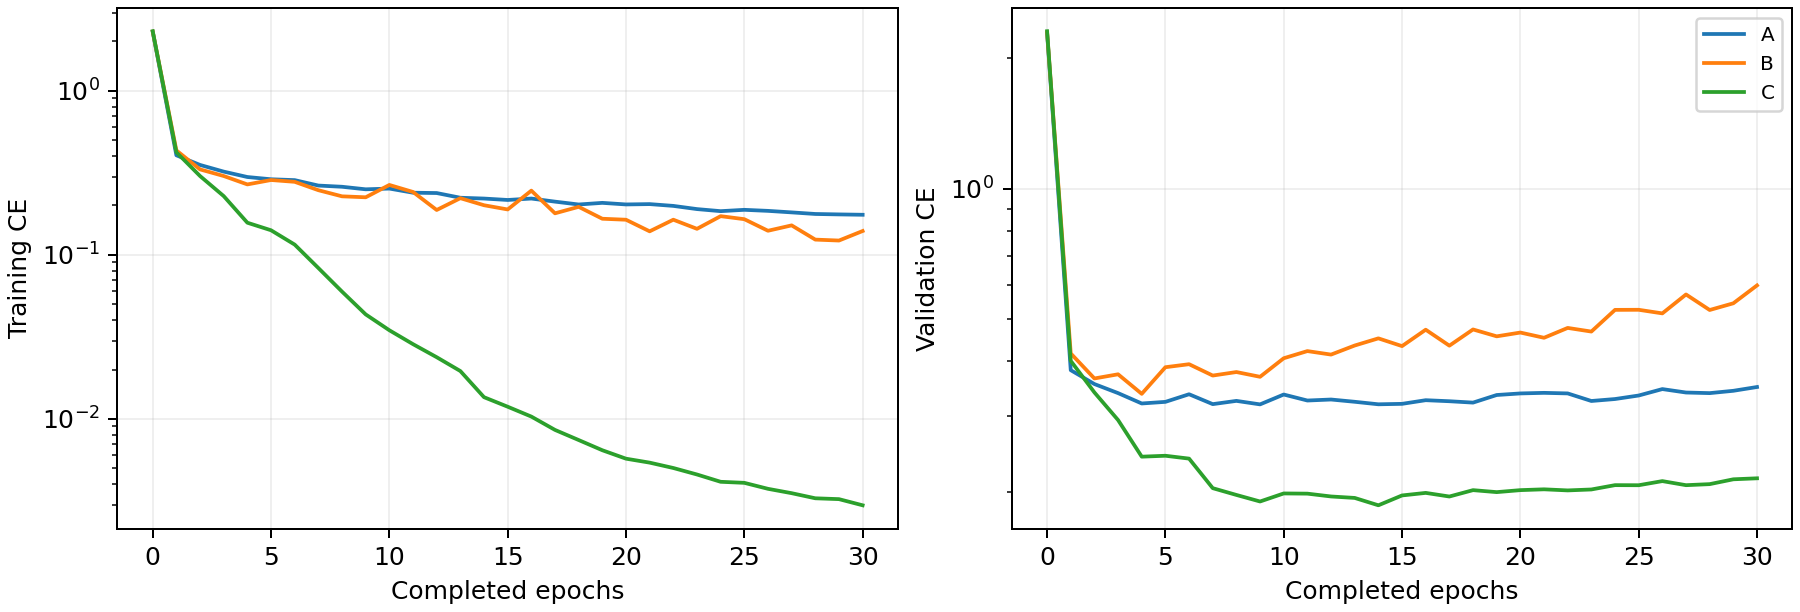
\includegraphics[width=\linewidth]{p3-curves.png}
\captionof{figure}{Training and validation cross-entropy (CE) for A, B and C. The supplied plotting code uses logarithmic vertical axes.}
\end{center}
\begin{center}
\begin{tabular}{crrrr}
\toprule
Model & Selected epoch & Validation CE & Test CE & Test accuracy\\
\midrule
A & 9 & 0.318305 & 0.277242 & 91.45\%\\
B & 4 & 0.336629 & 0.290094 & 90.80\%\\
C & 14 & 0.186219 & 0.170503 & 95.20\%\\
\bottomrule
\end{tabular}
\end{center}
\textbf{Validation choice.} C is preferred because its selected checkpoint has the smallest validation CE, $0.186219$. The reported test values are evaluations of each model's validation-selected state; test accuracy was not the selection criterion.

\textbf{A versus B.} B has slightly worse selected validation and test CE than A in this run, despite having more parameters and lower final training CE. This is consistent with the prediction that stacking affine layers does not enlarge the input-to-logit function class: factorizing the weights changes how optimization proceeds, so equivalent function classes need not yield equal trained solutions.

\textbf{B versus C.} With the same 50,890 parameters and identical layer dimensions, C lowers selected validation CE from $0.336629$ to $0.186219$ and raises test accuracy from $90.80\%$ to $95.20\%$. This supports the predicted usefulness of the hidden nonlinearity in this fixed experiment. It does not prove that ReLU always wins across data splits or seeds, and an A--C difference alone would mix activation and parameter-count effects.

\textbf{Training--validation gaps and checkpoint selection.}
\begin{center}
\small
\begin{tabular}{crrrr}
\toprule
& \multicolumn{2}{c}{Selected epoch} & \multicolumn{2}{c}{Epoch 30}\\
\cmidrule(lr){2-3}\cmidrule(lr){4-5}
Model & Training CE & Validation CE & Training CE & Validation CE\\
\midrule
A & 0.251042 & 0.318305 & 0.175604 & 0.349079\\
B & 0.268865 & 0.336629 & 0.139791 & 0.598827\\
C & 0.013566 & 0.186219 & 0.002974 & 0.214923\\
\bottomrule
\end{tabular}
\end{center}
All three models end with lower training CE but higher validation CE than at their selected epochs. B's validation curve rises most strongly, while C's training CE approaches zero without a matching late validation improvement. This widening gap is evidence of overfitting in this run; restoring the earlier validation minimum avoids simply taking a later, better-fitting training state. Validation selection is still an estimate from one finite split, not a guarantee of the best unknown population or test loss.

\clearpage
\section*{Problem 3(d): Actual coding-agent collaboration}
\textbf{Tool and scope.} OpenAI Codex was used in the desktop app for model construction, numerical checks, experiment execution and report drafting. The assistant identifies itself as GPT-6; no more specific model version is asserted here. The case below describes this actual interaction, rather than a fabricated student debugging exchange.

\textbf{Actual user prompt.} The initial Chinese request, translated into English, was:
\begin{quote}
\textquotedblleft Please help me complete hw03; you may refer to the completion format of previous assignments and AGENTS.md.\textquotedblright
\end{quote}
After the correct assignment files were supplied, the user asked, \textquotedblleft Now take another look.\textquotedblright\ The task then included the three model-construction functions required by Problem 3(b).

\textbf{Relevant agent reply.} Before running the experiment, Codex stated the following construction plan (translated from the original Chinese response):
\begin{quote}
\small\raggedright
\textquotedblleft The concrete implementations are \texttt{Linear(784,10)}, \texttt{Linear(784,64) $\to$ Linear(64,10)}, and \texttt{Linear(784,64) $\to$ ReLU $\to$ Linear(64,10)}; all outputs remain raw logits.\textquotedblright
\end{quote}
It also recorded that two layers without an activation remain affine, whereas hidden ReLU enables nonlinear piecewise-affine maps. The three actual return statements in the submitted \texttt{p3/p3.py} implement these definitions using \texttt{nn.Linear} and \texttt{nn.Sequential}.

\textbf{How the proposal was checked.} The checks were executed by the assistant, not presented as checks personally performed by the student. The provided framework reported:
\begin{center}
\begin{tabular}{ccc}
\toprule
Model & Trainable parameters & Output shape\\
\midrule
A & 7,850 & $(2,10)$\\
B & 50,890 & $(2,10)$\\
C & 50,890 & $(2,10)$\\
\bottomrule
\end{tabular}
\end{center}
The additional model tests passed: they checked the exact sequence of layer types, all biases, output dimensions and B's equality to its collapsed affine map within $10^{-12}$ in float64. Together with inspection of the constructors, these checks rule out an unintended output Softmax, missing bias or misplaced activation.

\textbf{Decision and evidence.} The proposed constructors were retained because the definitions, counts and checks agree with the three required formulas. No model-construction bug or artificial repair is claimed. The finite outputs and completed fixed-framework run provide execution evidence; they do not replace the algebra explaining A/B equivalence. The original interaction is retained in this Codex chat, and the local pre-run note and check logs preserve the timing and evidence.

\textbf{Authorship disclosure.} The mathematical explanations and this report are AI-assisted drafts. The numerical results come from actual local execution of the submitted implementation. The student remains responsible for checking understanding and expressing the derivations and explanations in their own words before submission; this record does not claim that personal step has already occurred.

\end{document}
